\section{Experimental}

\subsection{Samples}

All samples has been etched with an etch that consists of hydrofluoric acid, acetic acid, and nitric acid (HF:CH$_3$COOH:HNO$_3$) in a volume ratio of 36:15:2 known as Sopori etch \cite{soporietch}. This is done in order to bring dislocations to the surface. The sample name is constructed with ingot name first, sample preparation where Q3 denote wafers, and lastly, wafer number corresponding to a specific height in the ingot.

\begin{table}[H]
\centering
\begin{tabular}{|c|m{6cm}|c|}
\hline
\textbf{Name} & \textbf{Description} & \textbf{Feedstock} \\ \hline
R6-Q3-210 & Polysilicon, electronic grade, clean feedstock & Siemens process \\ \hline
ES1-Q3-201 & Large amount of P and B, solar grade, dirty feedstock & From Elkem \cite{hystad09} \\ \hline
MH2-Q3-210 & Same as ES1 with added Cr, solar grade, dirty feedstock & From Elkem \cite{hystad09} \\ \hline
\end{tabular}
\caption{Samples}
\label{tab:samples}
\end{table}

\subsubsection{R6-Q3-210}

This sample is from a clean feedstock, with low amount of impurities. B,Al and Fe where measured by Glow-Discharge Mass Spectrometry (GDMS), O and C where measured by Fourier transform infrared spectroscopy (FTIR). 

\begin{table}[H]
\centering
\begin{tabular}{|c|c|c|}
\hline
\textbf{Impurity} & \textbf{ppbw} & \textbf{atoms/cm$^3$} \\
\hline
B & 112.01 & 1.45\cdot10$^{16}$ \\ \hline
Al & 19.48 & 1.0\cdot10$10^{15}$ \\ \hline
Fe & nd & nd \\ \hline
C & 2576 & 2.26\cdot10$^{17}$ \\ \hline
O & 1932 & 8.87\cdot10$^{16}$ \\ \hline 
\end{tabular}
\caption{Impurities in R6 from \cite{chiara10}}
\label{tab:r6_impurities}
\end{table}

The impurities that are not listed were not analyzed, and are expected to be present in very low levels (tenths of ppbw).

\subsubsection{ES1-Q3-201}

This is a regular solar grade sample which originate from a compensated feedstock from Elkem Solar, from 90\% ingot height. Impurities are given by plot in \cite{hystad09}. Boron contaminants is between 550 and 700~ppbw, which corresponds to 7.1\cdot$10^{16}$ and 9.7\cdot$10^{16}$~atoms/cm$^3$ respectively using equation \ref{eq:ppbw}, and are homogenously distributed. Phosphorus is measured to be around 1200-1500~ppbw, which corresponds to 5.4-6.8\cdot$10^{16}$~atoms/cm$^3$.
Aluminum contaminants is just below 2.6\cdot10$^{15}$~atoms/cm$^3$. Other contaminants like Ti and Fe have very low values: less than 1.2\cdot$10^{14}$ and 3.8\cdot$10^{14}$~atoms/cm$^3$ respectively. For the lighter atom impurities, O have 1.7\cdot10$^{17}$~atoms/cm$^3$ and C have 6\cdot10$^{17}$~atoms/cm$^3$ \cite{hystad09}.

\subsubsection{MH2-Q3-210}

This sample is almost identical to ES1, but this sample have extra chromium added. Chromium contaminants is between 2 and 5 ppbw \cite{hystad09} which corresponds to 5.4\cdot$10^{13}$ and 1.3\cdot$10^{14}$~atoms/$cm^3$ respectively using equation \ref{eq:ppbw}, but exact concentration might be a little lower due detection limit of the instrument.


\subsection{Instrumentation}

\begin{figure}[H]
\centering
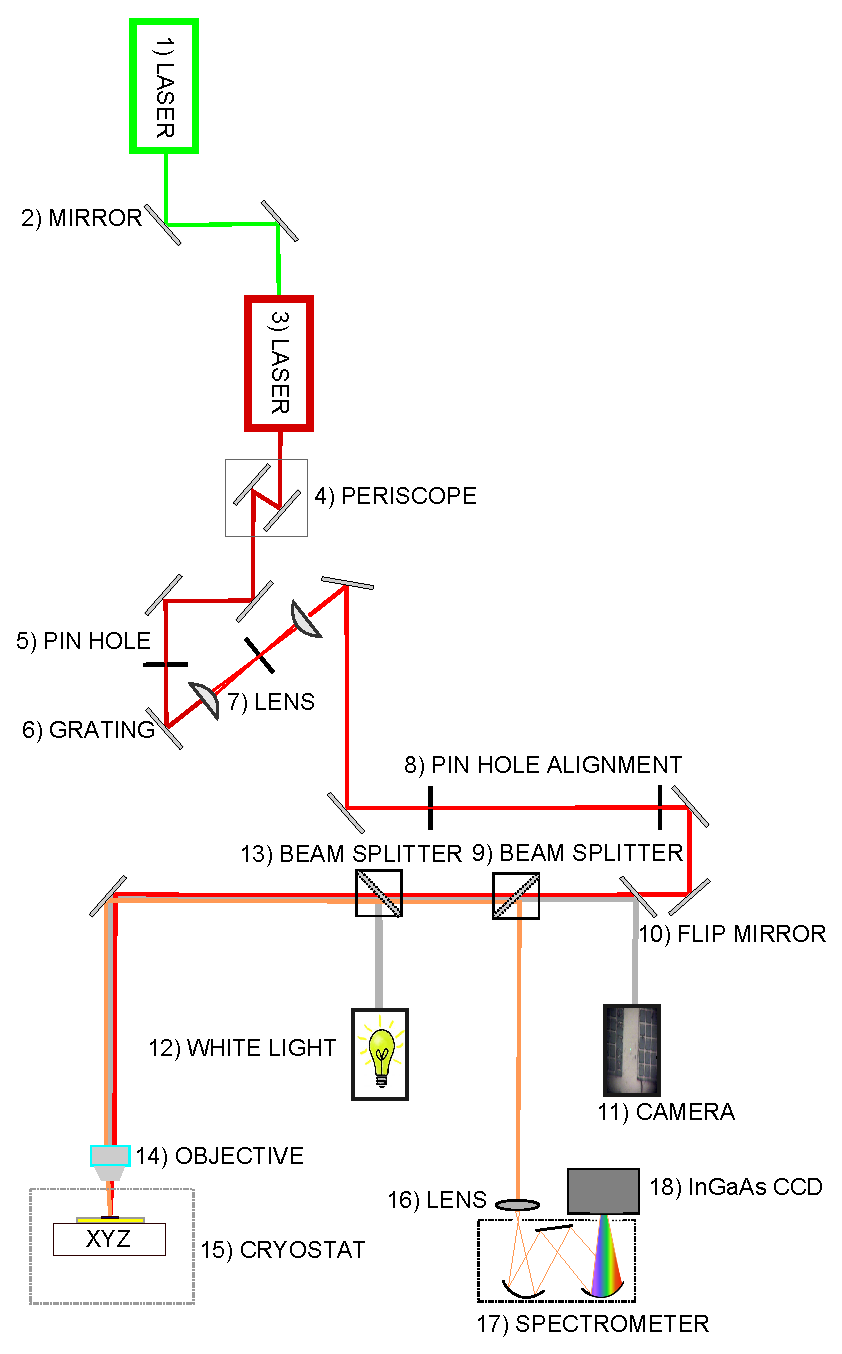
\includegraphics[width=0.8\columnwidth]{full_setup}%
\caption{Lab setup}%
\label{fig:full_setup}%
\end{figure}

\subsubsection{Optical components}

Optical components have been chosen to maximize luminescence light transmission of wavelengths 1.0-1.5~$�$m. This is because the silicon luminescence is known to be at these wavelengths (See table \ref{energy_bands}). The focusing lens in front of the spectrometer has above 90\% transmission for these wavelengths, according to its spesifications. As for the objective, it has 50X magnification, numerical aperture of 0.65, and a transmission curve that shows around 60\% transmission for these wavelengths according to datasheet, with a working distance of 10~mm. Mirrors have very wide spectral coverage and are completely achromatic.

The beam splitter in figure \ref{fig:full_setup}~\#10 transmits 90~\% of light from 400~nm to 2400~nm and is only used to shine white light on the sample in order to see where on the sample the laser spot is hitting. The white light source can easily be made strong enough, so that 10~\% reflectance is sufficient. As for the beam splitter in figure \ref{fig:full_setup}:9, it splits the light 50/50 in transmission and reflectance. This beam splitter is optimized for 1100-1600~nm with a splitter ratio tolerance less than 15~\% over the entire wavelength range. However 50~\% of the luminescence light from the sample is lost in the beam splitter, due to the split process.

\begin{table}[H]
\centering
\begin{tabular}{|c|c|c|c|}
\hline
\textbf{\#} & \textbf{Part} & \textbf{Product \#} & \textbf{Manufacturer} \\
\hline
1 & 532nm laser & YVO$_4$Nd$^{3+}$ & Spectra physics \\ \hline
2 & Metallic mirror & PF10-03-P01-10 & Thorlabs \\ \hline
3 & 800nm laser & Ti-sapphire Model 3900S & Spectra Physics \\ \hline
4 & Periscope & Two mounted mirrors & Thorlabs \\ \hline
5 & Pin hole & ID12SS/M & Thorlabs \\ \hline
6 & Grating & 23M27 &  \\ \hline
7 & Lens & AC254-150-B & Thorlabs \\ \hline
9 & Beam splitter & BS018 & Thorlabs \\ \hline
13 & Beam splitter & BP208 & Thorlabs \\ \hline
14 & Objective & NT56-982 & Mitutoyo \\ \hline
15 & Cryostat & Janis ST-500 & Janis Research Company \\ \hline
16 & Lens & LB4330 & Thorlabs \\ \hline
17 & Spectrometer & iHR550 Imaging Spectrometer & Horiba Scientific \\ \hline
18 & Camera & iDUS InGaAs Spectroscopy CCD 491-1.7& Andor Technology \\ \hline
\end{tabular}
\caption{Lab setup optical components}
\label{tab:lab_setup}
\end{table}



%% Spacial resolution, spectral resolution

\subsubsection{Pumping wavelength}

\cite{lee09} report that small angle grain boundaries in multicrystalline silicon of 1$^\circ$-1.5$^\circ$ show D3 and D4 lines, while 2$^\circ$-2.5$^\circ$ show D1 and D2 lines. Data from electron beam induced current measurements, show D1 and D2 lines to be correlated with shallow levels, while D3 and D4 appear in both shallow and deep levels \cite{lee09}.

The samples are pumped with a tunable Ti-sapphire laser, where a range of excitation wavelengths are available. A wavelength of 800 nm is chosen for excitation. This corresponds to an absorption depth of 12~$�$m in silicon \cite{laserdybde}. 800~nm is visible to the naked eye at high intensities, unlike larger wavelengths, which would make it much more difficult to align the setup, and make sure nothing is blocking the pathway. In the case of imperfect filtering of the reflected laser beam in front of the spectrometer, 800~nm (1.55eV) and the second order diffraction maxima at 1600~nm (0.775~eV), would be outside the most interesting wavelengths from silicon luminescence, and thus not influence the result (see table \ref{energy_bands} for silicon energy bands).

\subsubsection{Spot size}

For the setup given here, the spot size is around 2~$�$m. This is given by the magnification of the objective, and the diameter of the incoming laser beam. With this spot size, it is possible to detect micro-defect, like iron precipitates \cite{gundel09}. The downside to having such a small spot size, is the potential buildup of electron-hole drops for small volumes \cite{satoshi04}. This limitation can be overcome by using a larger wavelength, to excite a larger volume in the sample.
%% Due to the choise of optical components chosen, and be able to detect micro-defects .. lala .. cite - smallest possible by components

\subsubsection{Laser intensity}
% As large as possible, due to no EHD (as seen by experiment), and low temperature - larger signal to noise ratio - fill every single avaiblie state.
A high signal to noise ratio, is desirable. This is achieved by exciting with as much laser intensity as possible. As long as issues with electron-hole drops and temperature are negligible, the intensity can be quite high. The maximum laser intensity achieved in this setup is 128~mW of excitation intensity reaching the sample. A high intensity is also desirable to be able to fill every available electron state. With low intensities, only the most probable states will be visible in the luminescence specter.

\subsubsection{Temperature}

To achieve a high spectral resolution of the luminescence signal, it is needed to cool down the sample. Without cooling, the increased number of phonon states leads to energy broadening of the signal. This result in weaker signals not getting resolved, due to broadening of the strong signals, and thus overshadow the weaker signals. To reach temperatures of about 10~K, liquid helium is used for cooling. Liquid helium is introduced into the cryostat chamber, where it evaporates, drawing energy from its environment. The sample is on top of a sample holder, which is connected by copper wires to the cooling chamber, and a temperature readout. At such low temperatures, even weak signals as the ideally forbidden zero phonon recombination in silicon is visible \cite{davies88}.


\subsubsection{Spectrometer}

The spectrometer has a fixed grating, in front of InGaAs camera. The grating is 76~mm x 76~mm, with a groove density of 300. The camera consist of a single array of pixels. The full array of pixels detect wavelengths with a range of 140~nm, with 0.1~nm sensitivity, and is operated at -75$^\circ$C to minimize dark current noise. To measure a larger wavelength spectra than 140~nm, multiple measurements are needed at different wavelength intervals. The camera spectral response is from 0.8 to 1.7~$�$m, which is suitable for silicon photoluminescence.


